% This file was created by matlab2tikz v0.4.7 running on MATLAB 8.3.
% Copyright (c) 2008--2014, Nico Schlömer <nico.schloemer@gmail.com>
% All rights reserved.
% Minimal pgfplots version: 1.3
% 
% The latest updates can be retrieved from
%   http://www.mathworks.com/matlabcentral/fileexchange/22022-matlab2tikz
% where you can also make suggestions and rate matlab2tikz.
% 
%
% defining custom colors
\definecolor{mycolor1}{rgb}{0.00000,1.00000,1.00000}%
\definecolor{mycolor2}{rgb}{1.00000,0.00000,1.00000}%
\definecolor{mycolor3}{rgb}{0.83,0.69,0.22}%
%

\pgfplotsset{every axis label/.append style={font=\scriptsize
},
every tick label/.append style={font=\scriptsize
}
}




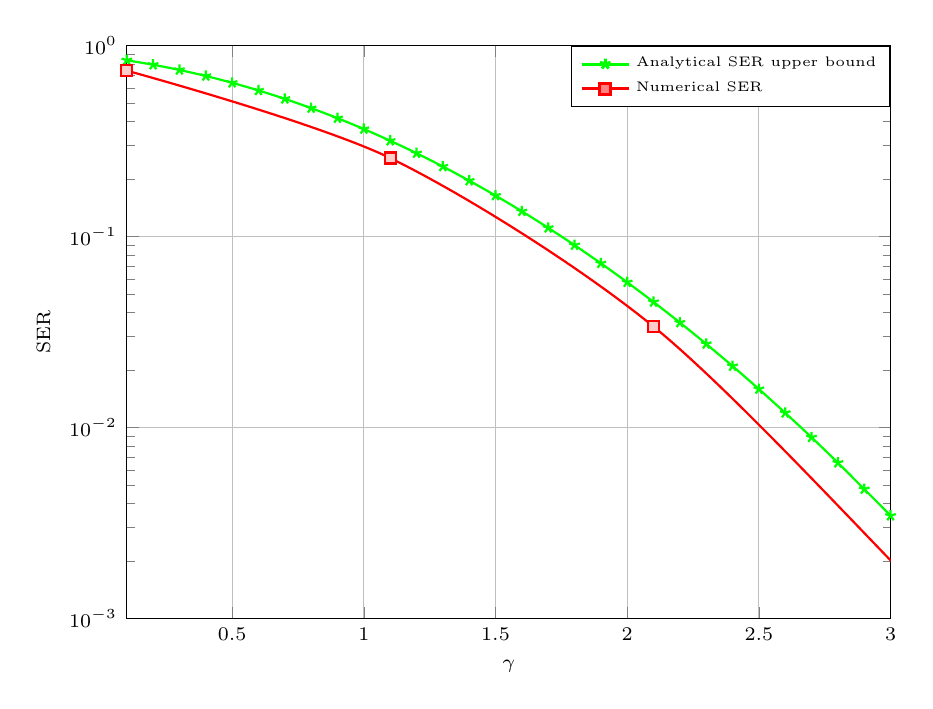
\begin{tikzpicture}[font=\scriptsize
] 
\begin{axis}[%
name=IF1,
%width=0.85\columnwidth,%5.63489583333333in,
width=0.8\columnwidth,
height=0.6\columnwidth,%4.16838541666667in,
scale only axis,
ymode=log,
xmin=0.1,
xmax=3,
xlabel={$\gamma$},
xmajorgrids,
ymin=0.001,
ymax=1,
ylabel={SER},
ymajorgrids,
legend entries={Analytical SER upper bound,  Numerical SER},
legend style={at={(1,1)},anchor=north east,draw=black,fill=white,legend cell align=left,font=\tiny}
]

%% Add a (b) below x-axis
%\pgfplotsset{
%    every axis/.append style={
%        extra description/.code={
%            \node at (0.5,-0.25) {(a)};
%        },
%    },
%}

%thick
\addlegendimage{smooth,color=green,solid, line width=1.1pt, mark=star,
y filter/.code={\pgfmathparse{\pgfmathresult-0}\pgfmathresult}}
\addlegendimage{smooth,color=red, solid, line width=1.1pt, every mark/.append style={solid, fill=red!50}, mark=square*,
y filter/.code={\pgfmathparse{\pgfmathresult-0}\pgfmathresult}}


%\addlegendimage{no markers}
%\addlegendimage{no markers,color=blue}
%\addlegendimage{no markers,color=red}
%\addlegendimage{no markers,color=black}




%\node [draw,fill=white,font=\tiny,anchor= %north east] at (axis cs: 20, 0.5 ) { %$M_{\text{Tx}} = M_{\text{Rx}}= 2$ };
%borrar

%  0.1	0.830594410875438\\
%0.2	0.784309082744384\\
%0.3	0.733119364270609\\
%0.4	0.67829479349396\\
%0.5	0.621347562543179\\
%0.6	0.563497424627338\\
%0.7	0.506015571178479\\
%0.8	0.449877142337167\\
%0.9	0.396094295268169\\
%1	0.345327539806263\\
%1.1	0.29818357870922\\
%1.2	0.254999162920816\\
%1.3	0.216015104681713\\
%1.4	0.181239262779404\\
%1.5	0.150660007371108\\
%1.6	0.124039368510162\\
%1.7	0.101174148805985\\
%1.8	0.0817352935896231\\
%1.9	0.0654403069459961\\
%2	0.051871269641007\\
%2.1	0.0407561725448982\\
%2.2	0.0317104336000321\\
%2.3	0.0244072957514507\\
%2.4	0.0186349094755488\\
%2.5	0.0140975719078485\\
%2.6	0.0105517378287425\\
%2.7	0.0078440994812039\\
%2.8	0.00574537573550493\\
%2.9	0.00418487443560156\\
%3	0.00300110287421762\\
%3.1	0.00214090391832711\\
%3.2	0.00152573745607176\\
%3.3	0.00107025975381825\\
%3.4	0.000747234857360946\\
%3.5	0.000520585658641437\\
%3.6	0.00034759829368558\\
%3.7	0.000240938406534941\\
%3.8	0.00014826814373281\\
%3.9	0.000104041121012255\\
%4	6.65939377884062e-05\\
%  }
%analytical 
\addplot+[smooth,color=green,solid, thick, every mark/.append style={solid, fill=gray!20} ,mark=star, mark repeat=1,
y filter/.code={\pgfmathparse{\pgfmathresult-0}\pgfmathresult}]
  table[row sep=crcr]{%
0.1	0.837189429663452\\
0.2	0.793552626330848\\
0.3	0.745070718618052\\
0.4	0.692837479889548\\
0.5	0.638101713681151\\
0.6	0.582037874205629\\
0.7	0.525742702659074\\
0.8	0.470292261211184\\
0.9	0.416576136747105\\
1	0.365400030127176\\
1.1	0.317372705181036\\
1.2	0.272965039589865\\
1.3	0.232501986902653\\
1.4	0.196098805431079\\
1.5	0.163821035051654\\
1.6	0.135516546523628\\
1.7	0.110996187105096\\
1.8	0.0900751011684547\\
1.9	0.0723692509246405\\
2	0.0575932084370129\\
2.1	0.0453775706225172\\
2.2	0.0354210562910303\\
2.3	0.0273688045842654\\
2.4	0.0209530363652815\\
2.5	0.0158856477202276\\
2.6	0.0119197714225323\\
2.7	0.00887462826109586\\
2.8	0.00653322775250631\\
2.9	0.0047532909564254\\
3	0.00344833973332281\\
3.1	0.00243362789572887\\
3.2	0.00172866144373462\\
3.3	0.00119646852018829\\
3.4	0.000848445812625442\\
3.5	0.000587127689037237\\
3.6	0.000403094161778195\\
3.7	0.000252692029805046\\
3.8	0.00018980641325439\\
3.9	0.000123641673068553\\
4	9.03194003791796e-05\\
};



%numerical MRx =2
\addplot+[smooth,color=red,solid, thick, every mark/.append style={solid, fill=red!20} ,mark=square*, mark repeat=1,
y filter/.code={\pgfmathparse{\pgfmathresult-0}\pgfmathresult}]
  table[row sep=crcr]{%
0.1	0.73875\\
1.1	0.25755\\
2.1	0.03375\\
3.1	0.00145\\
4.1	5e-05\\
};



%\addplot[smooth,color=green,solid, line width=1.1pt, %mark=none]
%  table[row sep=crcr]{%
%	50 2\\
%};\label{MC_MTX1}





%\node [draw,fill=white,font=\tiny,anchor= south west] %at (axis cs: -10, 0.1 ) {
%\setlength{\tabcolsep}{0.5mm}
%\renewcommand{\arraystretch}{.8}
%\begin{tabular}{l l}
%\ref{MC_MTX1}{$\; M_{\text{Rx}} =2$} \\
%\ref{MC_MTX2}{$\; M_{\text{Rx}} =3$} \\
%\ref{P5_Zz}{ MMSE ACE iter $i_{\text{max}}=20$} \\
%\ref{P0_Zz}{ Optimal MMSE ACE QP \cite{LarsonB_2017} } \\
%\ref{P1_Zz}{ joint MMDDT } \\
%\ref{P4_Zz}{ MMSE} \\
%\end{tabular}
%};


\end{axis}



\end{tikzpicture}%